% !TeX program = xelatex
\documentclass[11pt,a4paper]{article}

\usepackage{custom}

\title{\textbf{Chasing the Moment of Impact}\\[4pt]
  \large Collision Detection and Iterative Contact Resolution on CPU and CUDA}
\author{Justin-Marian Popescu\\[2pt]\small Proiect GPGPU}
\date{}

\begin{document}
\pagenumbering{roman}
\maketitle
\thispagestyle{empty}

\begin{abstract}
Când o bilă lovește o cutie, simulatorul trebuie să găsească locul
contactului și să calculeze cum se schimbă viteza și rotația fiecărui
object. Raportul urmărește acest proces de la aplicarea gravitației
până la urma colorată din imagine. Exemplele numerice și fragmentele
din cod leagă formulele de implementarea C++ și de shaderele GLSL.
Aceleași patru scene au fost rulate pe CPU și CUDA. Toate cele
\(4\,560\) de perechi de pași comparate au avut hash-uri de stare
identice. În scena cu \(4\,000\) de objects, raportul dintre timpul
median pe CPU și cel pe CUDA a fost \(1{,}59\).

\smallskip
\noindent\textbf{Cuvinte-cheie}\quad rigid-body dynamics, collision detection, impulse, friction, CUDA, impact heatmap
\end{abstract}

\clearpage
\tableofcontents
\clearpage
\pagenumbering{arabic}

\section{De la cădere la impact}

Poziția arată unde se află centrul bilei. Viteza liniară arată în ce
direcție și cât de repede se deplasează, iar viteza unghiulară descrie
rotația în jurul centrului. Gravitația schimbă viteza pe durata
căderii. La lovire, simulatorul aplică un \emph{impulse}, adică o
schimbare a cantității de mișcare. Un impuls a cărui linie de acțiune
trece pe lângă centru poate pune object-ul în rotație. Termenul \emph{rigid body} desemnează un object căruia modelul îi păstrează forma în timpul acestor mișcări.

Proiectul \code{chasing-moment-of-impact} folosește un \emph{physics engine}
cu pas fix \(h\). La fiecare pas aplică forțele,
caută perechi apropiate, verifică formele, rezolvă contactele și
actualizează pozițiile și orientările. Viewer-ul desenează starea
rezultată. Figura~\ref{fig:demo} arată incinta și object-urile din
scenariul demonstrativ. Engine-ul folosește un nucleu comun C++,
un \emph{CPU backend} serial și un \emph{CUDA backend} paralel.

\begin{figure}[!htbp]
\centering
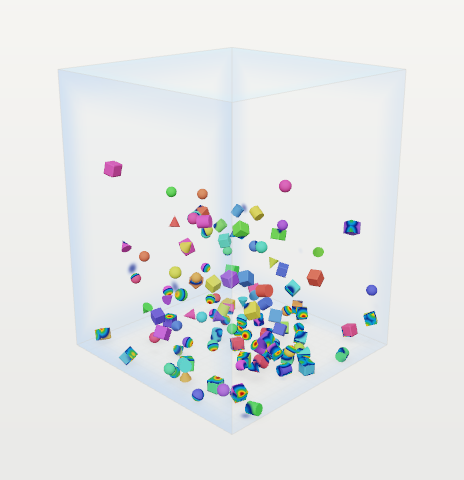
\includegraphics[height=43mm]{media/cuda-demo.png}%
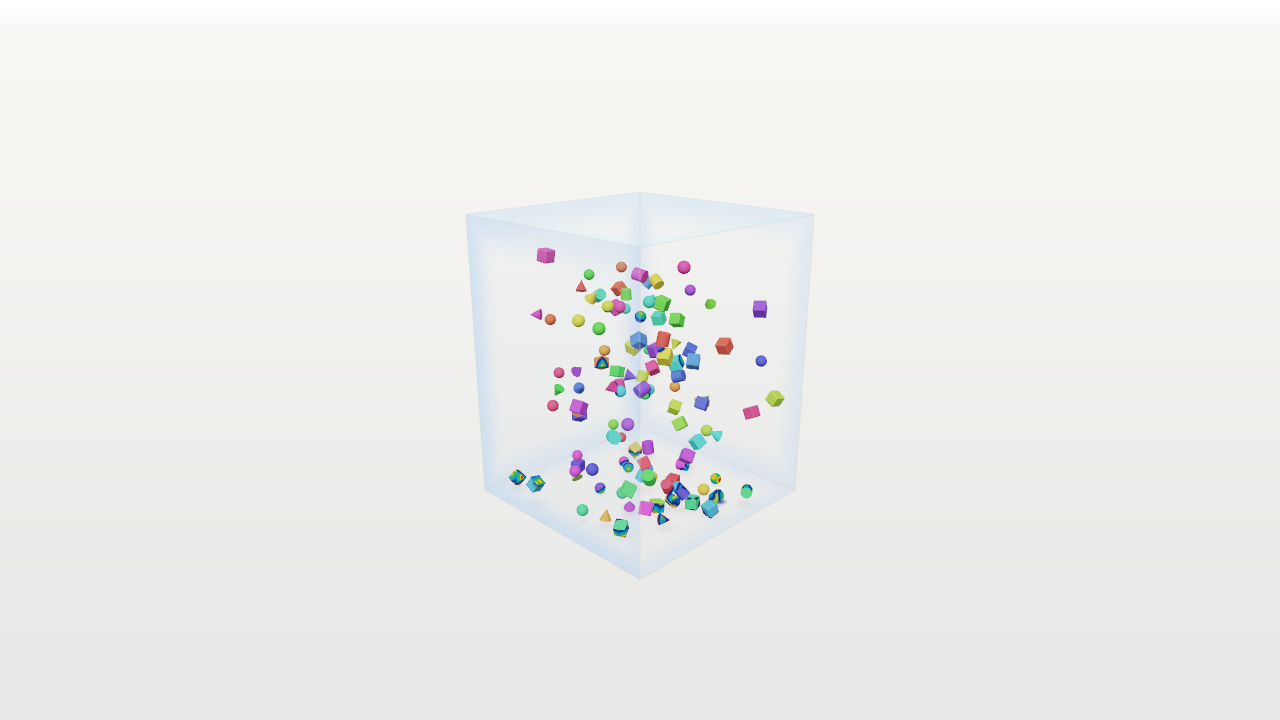
\includegraphics[height=43mm]{reports/run-cuda.png}
\caption{Objects de forme diferite în incintă. În stânga se vede
scenariul demonstrativ de aproape, iar în dreapta o rulare CUDA văzută
de la distanță.}
\label{fig:demo}
\imagecredit{\path{media/cuda-demo.png} (stânga) și \path{reports/run-cuda.png} (dreapta).}
\end{figure}

\section{Rigid-body state and dynamics}

\subsection{Position, orientation, mass, and inertia}

Un object este descris prin poziția centrului de masă \(\vect x\),
orientarea \(q\), \emph{linear velocity} \(\vect v\), \emph{angular velocity}
\(\vect\omega\), masa \(m\) și geometria de coliziune. Pozițiile sunt
în metri, vitezele liniare în \(\mathrm{m/s}\), vitezele unghiulare în
\(\mathrm{rad/s}\) și masele în kilograme. \emph{Linear momentum}
se calculează ca \(\vect P=m\vect v\), iar \emph{angular momentum}
față de centrul de masă este \(\vect L=I_w\vect\omega\).
Aici \(I_w\) reprezintă \emph{inertia tensor} exprimat în
\emph{world space}. Masa descrie rezistența la schimbarea
translației. Inerția descrie rezistența la schimbarea rotației și
depinde de axă și de distribuția masei.

Pentru o sferă omogenă de rază \(r\), valorile \emph{principal moments of inertia} sunt toate
\(\tfrac25mr^2\). Pentru o cutie de semidimensiuni
\((b_x,b_y,b_z)\), tensorul în axele proprii este diagonal, cu
\begin{equation}
  I_x=\tfrac m3(b_y^2+b_z^2),\quad
  I_y=\tfrac m3(b_x^2+b_z^2),\quad
  I_z=\tfrac m3(b_x^2+b_y^2).
\end{equation}
De exemplu, \(I_x=\int(y^2+z^2)\,\mathrm{d}m\), iar pentru distribuția
uniformă pe intervalul \([-b_y,b_y]\) media lui \(y^2\) este
\(b_y^2/3\). Engine-ul folosește un \emph{box collider} și pentru
cilindri și conuri. Dacă \(Q\) transformă axele locale în \emph{world space},
\(I_w^{-1}=Q I_{\mathrm{local}}^{-1} Q^\mathsf T\). Valorile stocate
sunt \(m^{-1}\) și diagonala lui \(I_{\mathrm{local}}^{-1}\),
folosite direct la aplicarea impulsurilor.
Inițializarea acestor valori se găsește în \code{State::spawn}
(\coderef{src/shared/sim/state.cpp}{105--106, 137--147}).

\code{State} deține un \emph{structure of arrays} (SoA), cu câte un tablou pentru fiecare proprietate.
\code{StateView} oferă acces la aceleași date prin \emph{pointers}
pe CPU sau CUDA.
Contactele sunt înregistrări separate, cu doi indici, un punct,
o normală, adâncimea cu semn și impulsurile acumulate. Al doilea
indice este negativ când contactul este cu un perete static.
\begin{codefragment}{Același indice identifică datele de poziție, mișcare și orientare.}{src/shared/sim/state.h}{107--112}
\begin{lstlisting}[numbers=left,firstnumber=107]
/* Vector state and cached collision bounds. */
Vec3 *position_m{}, *velocity_mps{}, *angularVelocity_rad_s{};
Vec3 *halfExtents_m{}, *inverseInertia_kg_m2{}, *force_N{}, *aabbExtent_m{};

/* Rotation state. */
Quat* orientation{};
\end{lstlisting}
\end{codefragment}

Capacitatea implicită este de \(8\,192\) de objects, cu 128 de
candidați pe object și \(4\cdot128+6\cdot8=560\) de poziții în
tabloul de contacte, pentru maximum patru puncte per pereche și
opt colțuri pe fiecare față a incintei. Etapele din
tabelul~\ref{tab:pipeline} sunt executate în aceeași ordine pe CPU
și CUDA. Engine-ul raportează dacă lista de candidați este plină
sau dacă \emph{solver}-ul depășește limita de 256 de culori.

\begin{table}[!htbp]
\centering\small
\begin{tabularx}{\linewidth}{@{}r l X@{}}
\hline
& \textbf{Etapă măsurată} & \textbf{Operație} \\
\hline
1 & \code{applyForces}       & Resetează marcajele de contact și aplică gravitația. \\
2 & \code{integrateVelocity} & Integrează forța și amortizează vitezele. \\
3 & \code{computeAabb}       & Recalculează semidimensiunile în axele lumii. \\
4 & \code{broadPhase}        & Sortează cheile celulelor și caută perechi candidate. \\
5 & \code{narrowPhase}       & Testează perechile și construiește \emph{contact manifolds}. \\
6 & \code{generateContacts}  & Adaugă contactele cu fețele incintei. \\
7 & \code{solveContacts}     & Colorează contactele, aplică impulsuri iterativ, înregistrează impacturile și corectează suprapunerile. \\
8 & \code{integratePosition} & Avansează poziția și orientarea și aplică limitele incintei. \\
9 & \code{updateSleep}       & Actualizează starea de \emph{sleep} și pune vitezele la zero pentru object-urile care intră în această stare. \\
10 & \code{emitDiagnostics}  & Raportează energie, cantitate de mișcare, contacte și corecții. \\
\hline
\end{tabularx}
\caption{Ordinea etapelor unui pas de simulare.}
\label{tab:pipeline}
\end{table}

\subsection{Gravity, damping, and time integration}

Pentru un object activ, gravitația este
\(\vect F_g=-mgs_g\vect e_y\), unde \(s_g\) este factorul gravitațional
al object-ului. Din \(m\,\mathrm{d}\vect v/\mathrm{d}t=\vect F_g\) rezultă
o schimbare \(-hgs_g\) a vitezei verticale înainte de amortizare.
La \(g=9{,}81\,\mathrm{m/s^2}\), \(s_g=1\) și \(h=1/120\,\mathrm{s}\),
aceasta este aproximativ \(-0{,}082\,\mathrm{m/s}\) pe pas.
Gravitația aplicată în centru are moment nul față de acesta. Rotația
se modifică prin termenul de \emph{angular damping} și prin impulsurile de contact.

Notăm coeficienții de \emph{linear damping} și \emph{angular damping}
cu \(d_v\) și \(d_\omega\), ambii în \(\mathrm{s^{-1}}\).
Engine-ul actualizează vitezele astfel.
\begin{equation}
 \vect v^-=\frac{\vect v_k+h\vect F_g/m}{1+d_vh},
 \qquad \vect\omega^-=\frac{\vect\omega_k}{1+d_\omega h}.
 \label{eq:integrare-viteze}
\end{equation}
Factorul \(1/(1+dh)\) este pasul implicit pentru termenul de
amortizare, obținut din \(u^- - u^\ast=-hd\,u^-\), unde \(u^\ast\)
este valoarea înainte de amortizare. După ce solver-ul tratează contactele,
engine-ul deplasează centrul cu \(h\vect v^+\) de la poziția
corectată. Folosirea vitezei noi pentru poziție este caracteristica
metodei \emph{semi-implicit Euler}.
\begin{codefragment}{Adaugă accelerația și aplică amortizarea.}{src/shared/sim/dynamics.h}{81--85}
\begin{lstlisting}[numbers=left,firstnumber=81]
if (s.isSleeping[i]) return;

s.velocity_mps[i] += s.force_N[i] * (s.inverseMass_per_kg[i] * dt_s);
s.velocity_mps[i] = s.velocity_mps[i] / (1 + c.linearDamping_per_s * dt_s);
s.angularVelocity_rad_s[i] = s.angularVelocity_rad_s[i] / (1 + c.angularDamping_per_s * dt_s);
\end{lstlisting}
\end{codefragment}

\subsection{Quaternion rotation}

Un \emph{unit quaternion} \(q=(\vect q,q_w)\) codifică rotația. Pentru
axa unitară \(\vect a\) și unghiul \(\theta\),
\(q=(\vect a\sin(\theta/2),\cos(\theta/2))\). Un vector local
\(\vect r\) se rotește folosind partea vectorială a produsului
\(q\otimes(\vect r,0)\otimes q^\ast\), unde \(q^\ast\) este
conjugatul. Pentru \(p=(\vect p,p_w)\) și
\(q=(\vect q,q_w)\), \emph{Hamilton product} se scrie
\begin{equation}
 p\otimes q=
 \bigl(p_w\vect q+q_w\vect p+\vect p\times\vect q,\ 
        p_wq_w-\vect p\cdot\vect q\bigr).
\end{equation}
Engine-ul exprimă \emph{angular velocity} în \emph{world space}, astfel încât
incrementul de rotație se înmulțește din stânga. Pentru un pas mic,
\(\sin(\|\vect\omega^+\|h/2)\simeq \|\vect\omega^+\|h/2\).
De aici rezultă actualizarea aproximativă
\begin{equation}
 q_{k+1}=\operatorname{normalize}
 \left(q_k+\tfrac h2(\vect\omega^+,0)\otimes q_k\right).
\end{equation}
Normalizarea împarte cele patru componente la norma lor. La
\(6\,\mathrm{rad/s}\) și 120 de pași pe secundă, object-ul se rotește
cu aproximativ \(0{,}05\,\mathrm{rad}\), adică \(2{,}9^\circ\), într-un pas.
\begin{codefragment}{Calculează schimbarea orientării și normalizează quaternion-ul.}{src/shared/sim/quaternion.h}{81--83}
\begin{lstlisting}[numbers=left,firstnumber=81]
Quat d = Quat{omega_rad_s.x, omega_rad_s.y, omega_rad_s.z, 0} * q;
Real h = dt_s * Real(.5);
return normalize(Quat{q.x + d.x * h, q.y + d.y * h, q.z + d.z * h, q.w + d.w * h});
\end{lstlisting}
\end{codefragment}

După integrare se recalculează limitele object-ului și se aplică
proiecția în incintă. Implicit, un object aflat în contact poate intra
în starea de \emph{sleep} după 60 de pași sub pragurile de \(0{,}05\,\mathrm{m/s}\)
și \(0{,}05\,\mathrm{rad/s}\). Contactul cu un object activ care
depășește un prag de mișcare îl poate reactiva.

\subsection{Energy and diagnostics}

Pentru un object, \emph{Kinetic energy} include translația centrului și rotația. \emph{Gravitational potential energy} are ca reper podeaua.
\begin{align}
 E_{\mathrm{cin}}&=\tfrac12m\|\vect v\|^2+
                   \tfrac12\vect\omega\cdot I_w\vect\omega,\\
 E_{\mathrm{pot}}&=mgs_g(y-y_{\mathrm{podea}}),\qquad
 \vect P_{\mathrm{total}}=\sum_i m_i\vect v_i .
\end{align}
În cădere, energia potențială scade și viteza crește. Un impact
oblic poate transfera energie de la translație la rotație. Frecarea,
amortizarea și ricoșeurile inelastice pot reduce energia mecanică
măsurată. Pereții exercită impulsuri externe asupra ansamblului
de objects, deci cantitatea de mișcare totală a object-urilor se poate
schimba. Diagnosticul mai numără perechile candidate, contactele
și corecțiile la pereți și verifică valorile nefinite.
\begin{codefragment}{Adaugă energiile și cantitatea de mișcare la total.}{src/shared/sim/diagnostics.h}{56--58}
\begin{lstlisting}[numbers=left,firstnumber=56]
d.kineticEnergy_J += (mass * dot(s.velocity_mps[i], s.velocity_mps[i]) + angular) * HALF;
d.potentialEnergy_J += mass * c.gravity_mps2 * s.gravityScale_unitless[i] * (s.position_m[i].y + c.boxHalfExtents_m.y);
d.linearMomentum_kgmps += s.velocity_mps[i] * mass;
\end{lstlisting}
\end{codefragment}

\section{Collision detection}

\subsection{Broad phase and spatial grid}

Etapa \emph{broad phase} restrânge căutarea la vecinătatea fiecărui object. Centrul
\(\vect x\) intră în celula \(\vect c=\lfloor\vect x/L_{\mathrm{cell}}\rfloor\),
cu latura \(L_{\mathrm{cell}}\) și rotunjire în jos pe fiecare axă. Cu
\(B=2^{20}\), cheia din trei câmpuri de câte 21 de biți este
\begin{equation}
 K_{\mathrm{cel}}=2^{42}(c_x+B)+2^{21}(c_y+B)+(c_z+B)
\end{equation}
pentru coordonate reprezentabile. Pe CPU se sortează perechile
(cheie, indice). Pe CUDA, algoritmul \emph{stable radix sort} păstrează ordinea
indicilor pentru chei egale \cite{cub}. Astfel, cele două implementări
vizitează object-urile dintr-o celulă în aceeași ordine.

BDEngine2D folosește o grilă cu \emph{spatial hashing} pentru a
reduce numărul de perechi de testat în 2D. În acest proiect,
engine-ul folosește celule 3D și sortează cheile celulelor înainte
de a căuta în vecinătatea fiecărui object \cite{medium-grid}.

Dacă \(R_i\) este \emph{bounding radius} pentru object-ul \(i\), iar
\(R_{\max}\) și \(V_{\max}\) sunt cea mai mare rază, respectiv cea mai mare viteză din scenă,
căutarea include \(s_i\) celule în fiecare sens pe fiecare axă.
Cu \emph{continuous collision detection} (CCD) activ, marja
de deplasare este \(D_i=h(\|\vect v_i^-\|+V_{\max})\) pentru
căutarea în grilă și \(D_{ij}=h(\|\vect v_i^-\|+\|\vect v_j^-\|)\)
pentru perechea \(i,j\). Cu CCD dezactivat, ambele marje sunt zero.
\begin{equation}
 s_i=\max\!\left(1,\left\lceil
 \frac{R_i+R_{\max}+d_{\mathrm{slop}}+D_i}
      {L_{\mathrm{cell}}}\right\rceil\right).
\end{equation}
Termenul de viteză provine din limita
\(\|\vect v_j^--\vect v_i^-\|\leq\|\vect v_i^-\|+\|\vect v_j^-\|\).
Din fiecare celulă se rețin doar candidații cu \(j>i\), pentru a
examina fiecare pereche o dată, și cu
\begin{equation}
 \|\vect x_j-\vect x_i\|^2\leq
 \left(R_i+R_j+d_{\mathrm{slop}}+D_{ij}\right)^2.
\end{equation}
\(d_{\mathrm{slop}}\) este toleranța \emph{contact slop}. Cheile sortate permit
localizarea începutului fiecărei celule prin \emph{binary search}.
În scene aglomerate, numărul de candidați crește chiar dacă se
folosește grila.
\begin{codefragment}{Mărește raza de căutare cu distanța maximă de deplasare când CCD este activ.}{src/shared/sim/broad_phase.h}{135--138}
\begin{lstlisting}[numbers=left,firstnumber=135]
Real reach_m = s.boundingRadius_m[i] + maxRadius_m + c.contactSlop_m;
if (c.enableCcd) {
    reach_m += (length(s.velocity_mps[i]) + maxSpeed_mps) * dt_s;
}
\end{lstlisting}
\end{codefragment}

\subsection{Narrow phase and contact manifolds}

Pentru două sfere, \(\vect d=\vect x_b-\vect x_a\),
\(d_{\mathrm{contact}}=r_a+r_b-\|\vect d\|\) și
\(\vect n=\vect d/\|\vect d\|\) când centrele sunt distincte.
Două sfere cu raze de \(0{,}5\,\mathrm m\) și centre la
\(0{,}9\,\mathrm m\) se suprapun cu \(0{,}1\,\mathrm m\).
Punctul reprezentativ este
\(\vect p=\vect x_a+(r_a-d_{\mathrm{contact}}/2)\vect n\).
\begin{codefragment}{Calculează adâncimea din suma razelor și distanța centrelor.}{src/shared/sim/contacts.h}{35--40}
\begin{lstlisting}[numbers=left,firstnumber=35]
Vec3 d = s.position_m[b] - s.position_m[a];
Vec3 normal = normalize(d);

Real distance = length(d);
Real r = s.halfExtents_m[a].x + s.halfExtents_m[b].x;
Real depth = r - distance;
\end{lstlisting}
\end{codefragment}

Pentru o sferă și un \emph{oriented bounding box} (OBB), centrul sferei se
transformă în axele cutiei,
\(\vect z=Q^\mathsf T(\vect x_{\text{sferă}}-\vect x_{\mathrm{cutie}})\).
Punctul cel mai apropiat are componentele
\(p_j=\clip(z_j,-b_j,b_j)\). În exterior, distanța
\(\|\vect z-\vect p\|\) se compară cu raza. În interior, normala
se alege pe axa feței celei mai apropiate, determinată de
\(\min_j(b_j-|z_j|)\). În exterior, adâncimea este raza
minus distanța până la punctul apropiat. În interior, este
raza plus distanța până la fața aleasă. Punctul de contact
în \emph{world space} este \(\vect x_{\mathrm{cutie}}+Q\vect p\).
Cilindrii și conurile folosesc aceeași
aproximare geometrică prin cutie orientată.
Implementarea perechilor sferă--sferă și sferă--cutie se găsește
în \code{sphereSphere} și \code{sphereBox}
(\coderef{src/shared/sim/contacts.h}{32--71, 87--129}).
În engine-ul 2D descris de Deepankar Agrawal, testul cerc--AABB
folosește același pas de \emph{clamp} pentru punctul cel mai
apropiat. Aici calculul are loc în trei dimensiuni, în coordonatele
locale ale OBB-ului \cite{medium-clamp}.

Conform \emph{Separating Axis Theorem} (SAT), două OBB-uri pot fi separate pe una dintre cele 15 axe candidate:
trei normale ale fiecărei cutii și nouă produse vectoriale între
direcțiile muchiilor \cite{obb}. Axele aproape nule sunt omise, iar
celelalte sunt normalizate. Proiecția pe axa unitară \(\vect a\)
este un interval cu centru \(\vect a\cdot\vect x_i\) și
semilățime \(r_{i,\mathrm{proj}}\).
\begin{align}
 r_{i,\mathrm{proj}}(\vect a)&=\sum_{j=1}^3 b_{ij}|\vect a\cdot\vect u_{ij}|,\\
 d_{\mathrm{contact}}(\vect a)&=r_{a,\mathrm{proj}}(\vect a)+r_{b,\mathrm{proj}}(\vect a)-
        |(\vect x_b-\vect x_a)\cdot\vect a|.
\end{align}
Dacă \(d_{\mathrm{contact}}<-d_{\mathrm{slop}}\) pe o axă, intervalele sunt separate.
Altfel, engine-ul alege cea mai mică valoare a lui \(d_{\mathrm{contact}}\) și
orientează normala de la object-ul \(a\) spre object-ul \(b\).
\begin{codefragment}{Respinge perechea când proiecțiile sunt separate peste toleranță.}{src/shared/sim/contacts.h}{180--184}
\begin{lstlisting}[numbers=left,firstnumber=180]
Real overlap = projectRadius(s, a, axis) + projectRadius(s, b, axis) - absolute(dot(delta, axis));

if (overlap < -c.contactSlop_m) {
    return false;
}
\end{lstlisting}
\end{codefragment}

Un contact între două fețe poate fi reprezentat prin mai multe
puncte. Când normala se aliniază cu o față, engine-ul o alege ca
\emph{reference face} și aplică \emph{polygon clipping} pe
\emph{incident face}, folosind cele patru semiplane laterale.
Pentru o muchie cu distanțe cu semn \(d_0,d_1\) de
semne opuse, punctul de intersecție este
\(\vect p_0+\tfrac{d_0}{d_0-d_1}(\vect p_1-\vect p_0)\).
Rezultă până la patru puncte distincte, adică un \emph{contact manifold}. Când decuparea nu produce puncte utile, rămâne
contactul reprezentativ dintre punctele de sprijin. Perechile
cu o sferă produc un singur contact.
\begin{codefragment}{Aplică polygon clipping și limitează numărul de puncte.}{src/shared/sim/manifolds.h}{204--212}
\begin{lstlisting}[numbers=left,firstnumber=204]
count = clipPolygon(first, count, second, axes[ru], center, h[ru]);
count = clipPolygon(second, count, first, -axes[ru], center, h[ru]);
count = clipPolygon(first, count, second, axes[rv], center, h[rv]);
count = clipPolygon(second, count, first, -axes[rv], center, h[rv]);

int written = 0;

// Limit to max 4 manifold points for stability and performance.
int samples = count > 4 ? 4 : count;
\end{lstlisting}
\end{codefragment}

\subsection{Intersection tests}

Un \emph{axis-aligned bounding box} (AABB) se suprapune cu altul
atunci când intervalele lor se suprapun pe toate cele trei axe.
Pentru o cutie orientată cu matrice \(Q\), semidimensiunile
AABB sunt \(\vect b_{\mathrm{AABB}}=|Q|\vect b\), cu modul
aplicat element cu element. Grila folosește \emph{bounding radius},
iar contactele dintre objects folosesc sferele și OBB-urile
descrise mai sus. Cele două funcții de mai jos sunt teste geometrice
separate, verificate prin \emph{unit tests}.

\paragraph{\code{rayTriangle}.}
Funcția primește originea \(\vect o\), direcția \(\vect d\) și
vârfurile triunghiului \(\vect a,\vect b,\vect c\). Folosește
algoritmul Möller--Trumbore pentru a rezolva ecuația
\cite{moller-trumbore}.
\begin{equation}
 \vect o+t\vect d=\vect a+u(\vect b-\vect a)+v(\vect c-\vect a).
\end{equation}
Ponderile vârfurilor sunt \(1-u-v\), \(u\) și \(v\). Dacă una
dintre ele e negativă, punctul se află în afara triunghiului.
Funcția acceptă intersecția pe oricare dintre fețe, inclusiv la
muchii și vârfuri. Respinge cazurile în care determinantul este
aproape zero, cum se întâmplă când raza este paralelă cu planul.
La succes întoarce \code{true} și scrie parametrul \(t\) în
\code{distance\_m}. Acesta este distanța în metri dacă
\(\|\vect d\|=1\). Parametrul \(t\) trebuie să fie nenegativ
pentru ca punctul să se afle pe semidreapta dată.
Pentru triunghiul cu vârfurile \((0,0,0)\), \((1,0,0)\) și
\((0,1,0)\), raza din \((0{,}2;\,0{,}2;\,1)\) cu direcția
\((0,0,-1)\) atinge triunghiul la \(t=1\). Aceeași direcție
din \((2,2,1)\) intersectează planul în afara triunghiului.
Implementarea de ray tracing în C\# a lui Emre Safa Baltacı
folosește același test Möller--Trumbore \cite{medium-ray}.
\coderef{src/shared/sim/intersections.h}{53--75}

\paragraph{\code{triangleTriangle}.}
Funcția primește două triunghiuri în același sistem de coordonate
și întoarce \code{true} dacă testul SAT găsește suprapunere.
Proiectează vârfurile pe normalele celor două fețe, pe produsele
vectoriale dintre perechi de muchii și pe axele din plan construite
din normala și muchiile fiecărui triunghi. O singură axă cu
intervale disjuncte este suficientă pentru \code{false}. Axele din plan
separă triunghiurile coplanare când proiecția pe normala comună
coincide. Funcția ignoră axele aproape nule și respinge
triunghiurile degenerate, cu arie aproape zero. Returnează un
\code{bool} pentru suprapunere.

De exemplu, triunghiul cu vârfurile \((2,2,0)\), \((3,2,0)\)
și \((2,3,0)\) este coplanar cu triunghiul din exemplul de mai sus,
dar proiecțiile pe axa \(x\) sunt \([0,1]\) și \([2,3]\).
Testul întoarce \code{false}. Testele proiectului acoperă și
intersecția necoplanară, includerea unui triunghi coplanar și
respingerea unui triunghi degenerat.
\coderef{src/shared/sim/intersections.h}{86--133}
\coderef{tests/unit/test_main.cpp}{170--183}

\subsection{Continuous collision detection and wall contacts}

Între două instantanee, un object rapid poate trece dincolo de un
obstacol subțire. Pentru două sfere separate, engine-ul caută
\emph{time of impact}, când centrele ajung la distanța \(r=r_a+r_b\),
cu viteza relativă \(\vect w=\vect v_b^--\vect v_a^-\).
Din \(\|\vect d+t\vect w\|^2=r^2\) rezultă
\begin{align}
 A&=\vect w\cdot\vect w,\qquad B=\vect d\cdot\vect w,\qquad
 C=\vect d\cdot\vect d-r^2,\\
 At^2+2Bt+C&=0,\qquad t_\star=\frac{-B-\sqrt{B^2-AC}}{A}.
\end{align}
Engine-ul testează dacă perechea se apropie, dacă discriminantul
este nenegativ și dacă \(t_\star\in[0,h]\). Dacă da, folosește
normala la momentul estimat și generează contactul cu adâncime
zero pentru pasul curent.
\begin{codefragment}{Acceptă impactul estimat dacă are loc în pasul curent.}{src/shared/sim/contacts.h}{54--60}
\begin{lstlisting}[numbers=left,firstnumber=54]
Real impact_s = (-bb - Real(sqrt(discriminant))) / aa;
if (impact_s < 0 || impact_s > dt_s) {
    return false;
}

normal = normalize(d + relative * impact_s);
depth = 0;
\end{lstlisting}
\end{codefragment}

Pentru o față a incintei cu normala exterioară \(\vect n\)
și distanța \(H_f\) față de origine, un punct \(\vect p\) al
object-ului are adâncimea \(d_f=\vect n\cdot\vect p-H_f\).
Viteza punctului spre exterior este
\(u_f=\vect n\cdot(\vect v+\vect\omega\times(\vect p-\vect x))\).
Se folosește punctul de sprijin al sferei sau fiecare dintre
cele opt colțuri ale cutiei. CCD păstrează și \emph{speculative contacts} dacă \(d_f+hu_f\) prezice traversarea. Pentru
cutii se adaugă marja \(R\|\vect\omega\|^2h^2\) și se verifică
separat limita conservatoare bazată pe raza de încadrare și
deplasarea maximă. Perechile sferă--OBB și OBB--OBB dintre
objects sunt testate la pozițiile curente, astfel încât
verificarea continuă este parțială. Logica pereților se află
în \code{wallContact} și \code{wallVertexContact}
(\coderef{src/shared/sim/manifolds.h}{252--344}).

\section{Iterative contact solver}

\subsection{Relative velocity and effective mass}

Considerăm un contact în punctul \(\vect p\), cu \emph{unit normal}
\(\vect n\) dinspre \(a\) spre \(b\). Cu
\(\vect r_i=\vect p-\vect x_i\), viteza suprafeței object-ului \(i\)
în punctul de contact este
\(\vect v_i+\vect\omega_i\times\vect r_i\). Diferența dintre cele
două viteze este \emph{relative velocity},
\begin{equation}
 \vect u=(\vect v_b+\vect\omega_b\times\vect r_b)-
         (\vect v_a+\vect\omega_a\times\vect r_a),\qquad
 u_n=\vect u\cdot\vect n.
\end{equation}
Dacă \(u_n<0\), suprafețele se apropie. Un perete static are
viteza, masa inversă și inerția inversă egale cu zero în calcul.

Un impuls scalar \(J\) pe direcția unitară \(\vect d\)
schimbă viteza relativă proiectată pe acea direcție cu
\(J K(\vect d)\), unde \(K\) este \emph{inverse effective mass}.
\begin{equation}
 K(\vect d)=
 \sum_{i\in\{a,b\}}\!
 \left[m_i^{-1}+(\vect r_i\times\vect d)\cdot
       I_{i,w}^{-1}(\vect r_i\times\vect d)\right].
 \label{eq:inverse-effective-mass}
\end{equation}
Primul termen vine din translația centrului. Al doilea vine din
schimbarea vitezei unghiulare produsă de impuls. Într-adevăr,
\(\vect d\cdot(\Delta\vect\omega_i\times\vect r_i)=
\Delta\vect\omega_i\cdot(\vect r_i\times\vect d)\).
Dacă linia de acțiune trece prin centru, produsul vectorial este
zero și object-ul contribuie doar prin \(m_i^{-1}\). Într-o
lovitură frontală între două sfere, \emph{effective mass} coincide cu \emph{reduced mass} \(m_am_b/(m_a+m_b)\).

\begin{codefragment}{Contribuția unui object la \(K(\vect d)\) include masa inversă și termenul de rotație.}{src/shared/sim/solver.h}{27--30}
\begin{lstlisting}[numbers=left,firstnumber=27]
Vec3 ra = ct.point_m - s.position_m[ct.a_i];

// Linear inverse mass plus the angular contribution (r x axis) dot (I^-1 * (r x axis)).
Real result = s.inverseMass_per_kg[ct.a_i] + dot(axis, cross(inverseInertia(s, ct.a_i, cross(ra, axis)), ra));
\end{lstlisting}
\end{codefragment}

\subsection{Restitution and normal impulse}

La începutul pasului se calculează valoarea \emph{target velocity} \(u_\star\).
Dacă viteza normală inițială \(u_{n,0}\) este sub pragul negativ
de ricoșeu, ținta este \(-e\,u_{n,0}\), unde \(e\) este
\emph{coefficient of restitution}. Altfel, ținta este zero. Pentru un
\emph{speculative contact} cu adâncimea \(d_{\mathrm{contact}}<-d_{\mathrm{slop}}\),
solver-ul ia minimul dintre această țintă și \(d_{\mathrm{contact}}/h\). Această limită
permite apropierea cu cel mult distanța disponibilă într-un pas.

La fiecare iterație, solver-ul ajustează valoarea \emph{accumulated normal impulse}
\cite{catto}.
\begin{equation}
 J_n'=\max\!\left(0,J_n+
             \frac{u_\star-u_n}{K(\vect n)}\right),\qquad
 \Delta\vect J_n=(J_n'-J_n)\vect n .
\end{equation}
Proiecția pe valori nenegative permite contactului să împingă.
Incrementul poate avea semn negativ dacă o iterație anterioară
a aplicat un impuls prea mare. Object-ul \(a\) primește
\(-\Delta\vect J_n\), iar object-ul \(b\) primește
\(+\Delta\vect J_n\). Impulsurile se acumulează între iterațiile
aceluiași pas și pornesc de la zero pentru contactele nou generate.

Pentru o comparație cu un alt engine, Maciej Mizerski descrie
aplicarea impulsurilor în spațiul vitezelor și folosirea
\emph{Projected Gauss--Seidel} în Roblox. Același principiu apare aici
în actualizarea repetată a impulsului de contact. Ordinea pe culori
și execuția CUDA sunt detalii ale acestui proiect \cite{medium-roblox}.
\begin{codefragment}{Variabila \code{massInv} este \(K(\vect n)\). Se aplică diferența de impuls.}{src/shared/sim/solver.h}{138--145}
\begin{lstlisting}[numbers=left,firstnumber=138]
Real increment = (ct.targetVelocity_mps - dot(relative, ct.normal)) / massInv;
Real previous = ct.normalImpulse_Ns;

// Clamp the accumulated impulse to be non-negative (unilateral constraint).
ct.normalImpulse_Ns = maximum(0, previous + increment);

// Apply the normal impulse change.
applyImpulse(s, ct, ct.normal * (ct.normalImpulse_Ns - previous));
\end{lstlisting}
\end{codefragment}

\paragraph{Exemplu între două sfere.}
Sfera \(a\), de \(1\,\mathrm{kg}\), ajunge cu \(2\,\mathrm{m/s}\)
la sfera \(b\), care are aceeași masă și stă pe loc.
Pentru o lovitură pe linia centrelor,
\(K(\vect n)=2\,\mathrm{kg^{-1}}\). Cu \(e=0{,}5\), viteza de
separare dorită este \(1\,\mathrm{m/s}\). Impulsul calculat este
\((1-(-2))/2=1{,}5\,\mathrm{N\,s}\). Vitezele finale sunt
\(0{,}5\,\mathrm{m/s}\) și \(1{,}5\,\mathrm{m/s}\) în direcția
inițială a sferei \(a\). Cantitatea de mișcare totală rămâne
\(2\,\mathrm{kg\,m/s}\), iar energia cinetică scade de la
\(2\,\mathrm J\) la \(1{,}25\,\mathrm J\). Pentru contactul
izolat, fără frecare, energia pe direcția normală scade de la
\(E_n\) la \(e^2 E_n\). Diferența este \((1-e^2)E_n\).

\paragraph{Exemplu de cădere și ricoșeu.}
În modelul ideal fără amortizare, o bilă lăsată de la înălțimea
\(H\) ajunge la podea cu viteza \(\sqrt{2gH}\), din egalitatea
\(mgH=\tfrac12mv^2\). După o lovitură verticală, pleacă în sus
cu viteza \(e\sqrt{2gH}\) și atinge înălțimea \(e^2H\).
O cădere de un metru cu \(e=0{,}5\) produce un ricoșeu de
aproximativ 25 cm. Pasul finit și amortizarea pot schimba
această valoare în simulator. Pragul de viteză pentru \emph{restitution} ajută
contactele aproape în repaus să se stabilizeze.

\subsection{Angular impulse and friction}

Dacă \(\Delta\vect J\) este impulsul cu semn primit de un object,
\begin{equation}
 \Delta\vect P=\Delta\vect J,\qquad
 \Delta\vect L=\vect r\times\Delta\vect J,\qquad
 \Delta\vect\omega=I_w^{-1}\Delta\vect L.
\end{equation}
Modulul \emph{angular impulse} este
\(\|\vect r\|\|\Delta\vect J\|\sin\theta\), unde \(\theta\)
este unghiul dintre braț și impuls. Un impuls de
\(2\,\mathrm{N\,s}\) aplicat perpendicular la \(0{,}3\,\mathrm m\)
de centru produce \(0{,}6\,\mathrm{kg\,m^2/s}\) moment cinetic.
Dacă inerția pe axa respectivă este \(0{,}2\,\mathrm{kg\,m^2}\),
viteza unghiulară se schimbă cu \(3\,\mathrm{rad/s}\).
Engine-ul folosește viteza actualizată la integrarea orientării prin
\emph{quaternion rotation}.
\begin{codefragment}{Actualizează vitezele object-ului A. Object-ul B primește impulsul cu semnul opus.}{src/shared/sim/solver.h}{53--55}
\begin{lstlisting}[numbers=left,firstnumber=53]
// Update body A (subtract impulse).
s.velocity_mps[a] -= impulse_Ns * s.inverseMass_per_kg[a];
s.angularVelocity_rad_s[a] -= inverseInertia(s, a, cross(ct.point_m - s.position_m[a], impulse_Ns));
\end{lstlisting}
\end{codefragment}

După impulsul normal se recalculează viteza relativă și se
extrage alunecarea
\(\vect u_t=\vect u-(\vect u\cdot\vect n)\vect n\).
Pentru \(\|\vect u_t\|>0\), se alege direcția
\(\vect t=\vect u_t/\|\vect u_t\|\). Valoarea propusă pentru \emph{tangential impulse} este
\begin{equation}
 \vect J_t^{\mathrm{cand}}=
 \vect J_t-\frac{\vect u_t}{K(\vect t)}.
\end{equation}
Dacă modulul impulsului propus este cel mult \(\mu_sJ_n'\),
solver-ul îl acceptă. Dacă limita este depășită, solver-ul păstrează
direcția impulsului și îi reduce modulul la \(\mu_dJ_n'\).
Se aplică diferența față de impulsul tangențial deja acumulat.
Cu \(J_n'=2\,\mathrm{N\,s}\), \(\mu_s=0{,}5\) și
\(\mu_d=0{,}4\), limita pentru \emph{static friction} este \(1\,\mathrm{N\,s}\).
Dacă sunt necesari \(1{,}4\,\mathrm{N\,s}\) pentru oprirea
alunecării, limita pentru \emph{kinetic friction} este \(0{,}8\,\mathrm{N\,s}\).
\begin{codefragment}{Verifică limita statică și aplică limita cinetică dacă este depășită.}{src/shared/sim/solver.h}{165--172}
\begin{lstlisting}[numbers=left,firstnumber=165]
Vec3 proposed = ct.tangentImpulse_Ns - tangent * (speed / tangentMass);
Real magnitude = length(proposed);

// Apply Coulomb friction limit.
if (magnitude > c.frictionStatic_unitless * ct.normalImpulse_Ns) {
    // If static friction is exceeded, clamp to dynamic friction.
    proposed = normalize(proposed) * (c.frictionDynamic_unitless * ct.normalImpulse_Ns);
}
\end{lstlisting}
\end{codefragment}

Pe o bilă care alunecă pe podea, \emph{friction} acționează în
punctul de contact. Impulsul tangențial reduce alunecarea și poate
crește viteza unghiulară în sensul rulării. La \emph{rolling without slipping} pe un plan static,
\(\vect v+\vect\omega\times\vect r\) are componenta tangențială
nulă la contact. Pentru o bilă cu axa de rotație perpendiculară
pe direcția deplasării, aceasta dă \(\|\vect v\|=r\|\vect\omega\|\).

\subsection{Position correction}

Etapa \emph{position correction} se aplică separat de impulsuri. Pentru
\(w_i=m_i^{-1}\), \(d_{\mathrm{excess}}=\max(0,d_{\mathrm{contact}}-d_{\mathrm{slop}})\),
coeficientul de corecție \(k_{\mathrm{corr}}\) și factorul \(s_m\), deplasările sunt
\begin{equation}
 \Delta\vect x_a=-\frac{w_a}{w_a+w_b}k_{\mathrm{corr}} s_md_{\mathrm{excess}}\vect n,
 \qquad
 \Delta\vect x_b=+\frac{w_b}{w_a+w_b}k_{\mathrm{corr}} s_md_{\mathrm{excess}}\vect n.
\end{equation}
Object-ul cu masă mai mică se deplasează mai mult. Factorul
\(s_m=1/4\) la un contact OBB--OBB limitează corecția cumulată
a unui \emph{contact manifold} cu mai multe puncte. Pentru un contact cu
sferă se folosește \(1\). Contactele cutie--perete au o
corecție separată pe baza dimensiunilor cutiei. După avansarea
poziției și orientării, o proiecție finală limitează
centrul în funcție de semidimensiunile actualizate.
Valorile implicite sunt \(d_{\mathrm{slop}}=0{,}001\,\mathrm m\) și
\(k_{\mathrm{corr}}=0{,}6\). Sursa formulei este \code{correctContactPosition}
(\coderef{src/shared/sim/solver.h}{192--231}).

\section{CUDA execution and reproducibility}

Fiecare contact poate fi privit ca o muchie între object-urile pe
care le modifică. Contactele cu pereții au un singur object activ.
Algoritmul de \emph{graph coloring} parcurge contactele într-o ordine fixă și alege
pentru fiecare prima culoare liberă la object-urile implicate.
Contactele de aceeași culoare pot fi procesate în paralel,
fiindcă fiecare contact modifică alte objects. Culorile următoare văd vitezele
deja actualizate, ca într-o iterație Gauss--Seidel pe grupuri.

Pe CUDA, un singur \emph{thread} colorează contactele, iar solver-ul
rulează într-un \emph{thread block} cu 128 de threads. Fiecare thread
procesează o parte dintre contactele unei culori. Sincronizarea prin
\code{\_\_syncthreads()} are loc înainte
de următoarea culoare. CPU folosește aceeași ordine în mod
serial. Puține contacte într-o culoare lasă threads inactive,
iar mai multe culori înseamnă mai multe \emph{synchronization barriers}.
Un singur bloc limitează solver-ul la un \emph{streaming multiprocessor}
(SM). Etapa \emph{broad phase}, generarea contactelor și alte etape
folosesc mai multe blocuri. Maximele
globale pentru căutare, colorarea și diagnosticul rulează
serial pe dispozitiv.

\begin{codefragment}{Thread-urile tratează contactele aceleiași culori în paralel și se sincronizează înainte de culoarea următoare.}{src/physics/backend/cuda/solver.cu}{68--75}
\begin{lstlisting}[numbers=left,firstnumber=68]
for (int iteration = 0; iteration < c.solverIterations_i; ++iteration) {
    for (int color = 0; color < *number; ++color) {
        for (int k = offsets[color] + int(threadIdx.x); k < offsets[color + 1]; k += int(blockDim.x)) {
            solveContactConstraint(s, contacts[indices[k]], c);
        }
        __syncthreads();
    }
}
\end{lstlisting}
\end{codefragment}

CUDA backend-ul păstrează tablourile de stare pe GPU și
folosește spațiu CUB prealocat. Transferurile trec prin \emph{pinned host memory}. Copiile sunt programate asincron pe același \emph{CUDA stream}, cu sincronizare la limita apelului. Pasul
sincronizează și rezultatele de diagnostic. Viewer-ul și
executabilul de test cer separat descărcarea stării.
Timpii etapelor pe GPU se măsoară cu \emph{CUDA events}, iar pe CPU
cu un \emph{monotonic clock}. Timpul total include lansarea
operațiilor CUDA, copierea datelor de diagnostic și sincronizarea de la
sfârșitul pasului.

Ordinea perechilor și a culorilor este deterministă. Opțiunile
\code{/fp:strict} sau \code{-ffp-contract=off} pe CPU și
\code{--fmad=false} pe CUDA reduc diferențele aritmetice.
Executabilul salvează la fiecare pas un hash FNV-1a de 64 de
biți pentru numărul de objects, pas și câmpurile selectate
ale stării, inclusiv poziții, orientări, viteze și starea de \emph{sleep}.
La \emph{replay}, engine-ul încarcă starea inițială și configurația,
apoi compară fiecare pas cu \emph{trace}-ul salvat. Verificarea acoperă câmpurile
incluse în hash, pe scenele și configurația testate.

\section{Scene rendering and impact visualization}

\subsection{From physics state to rendered frame}

Viewer-ul primește starea după pasul de simulare. Pentru
fiecare formă refolosește același \emph{mesh} și îl desenează pentru mai multe objects prin \emph{instanced rendering}. Fiecare object are propria \emph{model matrix}
\(M=TQS\). Matricea \(M\) aplică fiecărui vârf local
transformările \emph{scale}, \emph{rotation} și \emph{translation}.
Rotația vine din quaternion-ul object-ului, iar translația din
poziția centrului. Programul \emph{vertex shader} aplică apoi matricea
de vizualizare \(V\) și proiecția camerei \(P\), în ordinea
\(\vect x_{\mathrm{clip}}=PVM\vect x_{\mathrm{local}}\).
\begin{codefragment}{Construiește transformarea object-ului prin scalare, rotație și translație.}{src/client/render_gl/rigid_bodies/draw_objects.cpp}{116--120}
\begin{lstlisting}[numbers=left,firstnumber=116]
// Column vectors apply scale first, then rotation, then translation into world space.
const auto model =
    glm::translate(glm::mat4(1.0f), glm::vec3(position_m.x, position_m.y, position_m.z)) *
    glm::mat4_cast(glm::quat(orientation.w, orientation.x, orientation.y, orientation.z)) *
    glm::scale(glm::mat4(1.0f), glm::vec3(halfExtents_m.x, halfExtents_m.y, halfExtents_m.z));
\end{lstlisting}
\end{codefragment}

Normala descrie orientarea unei suprafețe. La scalare
neuniformă, ea se transformă prin inversa transpusă a
părții liniare a matricei de model, pentru a rămâne
perpendiculară pe suprafață. Programul \emph{fragment shader} combină
culoarea de bază cu lumina principală, lumina de umplere,
lumina de contur și lumina ambientală. Termenul de \emph{diffuse lighting} este proporțional cu \(\max(0,\vect n\cdot\vect l)\), unde
\(\vect l\) indică direcția luminii. Termenul \emph{specular highlight} dă luciul. Culorile sunt comprimate prin \emph{ACES tone mapping} și convertite
în sRGB înainte de suprapunerea urmelor. Pereții
transparenți sunt desenați de la cel mai îndepărtat
la cel mai apropiat, după object-urile opace.

\subsection{Soft contact shadows}

Pentru un object cu raza de încadrare \(R\) și semidimensiunea
verticală AABB \(b_y\), distanța estimată până la podea este
\(a=y-y_{\mathrm{podea}}-b_y\). Engine-ul plasează o umbră
sub centrul object-ului, la 3 mm deasupra podelei, cu
\begin{equation}
F_{\mathrm{shadow}}=\clip\!\left(1-\frac{a}{3R},0,1\right).
\end{equation}
Umbra este mai intensă lângă podea. În timpul unui
ricoșeu, \(a\) crește și umbra se estompează până dispare.
Calculul se află în \code{buildShadows}
(\coderef{src/client/render_gl/rigid_bodies/draw_environment.cpp}{95--119}).

Shader-ul evaluează mai multe eșantioane dispuse pe o
\emph{golden-angle spiral}. Pentru coordonata locală \(\vect z\)
din umbră și deplasările \(\vect t_j\) ale eșantioanelor, opacitatea
este proporțională cu
\(F_{\mathrm{shadow}}\,N^{-1}\sum_j
 \exp(-k_{\mathrm{shadow}}\|\vect z+\vect t_j\|^2)\).
Media netezește marginea. Podeaua se desenează prima, astfel
încât umbra să întunece grila înainte de desenarea object-urilor.
\begin{codefragment}{Calculează opacitatea umbrei folosind factorul de fade din \code{visual.z}.}{src/client/render_gl/shaders/shadow.frag}{41--49}
\begin{lstlisting}[language=ReportGLSL,numbers=left,firstnumber=41]
    // Accumulate the exponential falloff based on the distance to the sample.
    sum += exp(-dot(p + tap, p + tap) * WORLD.SHADOW.SHADOW_FOOTPRINT_FALLOFF);
}

// Output the tint with the averaged shadow density as alpha.
fragmentColor = vec4(
    WORLD.SHADOW.SHADOW_TINT,
    WORLD.SHADOW.SHADOW_FOOTPRINT_STRENGTH * visual.z * sum / float(WORLD.SHADOW.SHADOW_TAP_COUNT)
);
\end{lstlisting}
\end{codefragment}

\subsection{Impact energy}

Înainte de rezolvare se măsoară componenta normală a vitezei
de apropiere. Folosind \emph{effective mass} \(1/K(\vect n)\),
\begin{equation}
 v_c=\max(0,-\vect u_0\cdot\vect n),\qquad
 E_n=\tfrac12\bigl(1/K(\vect n)\bigr)v_c^2 .
\end{equation}
\(E_n\) reprezintă energia de apropiere a unui contact pe
direcția normală. La aceeași masă efectivă, dublarea vitezei
înmulțește energia cu patru. Cele trei sfere din
figura~\ref{fig:impact} pornesc cu \(1\), \(4\) și \(9\,\mathrm{m/s}\),
cu gravitația și amortizarea dezactivate. Scena este definită
de \code{viewerScenario} și \code{populateViewer}
(\coderef{src/physics/scenarios/impact_demo.cpp}{22--35, 55--85}).

\begin{figure}[!htbp]
\centering
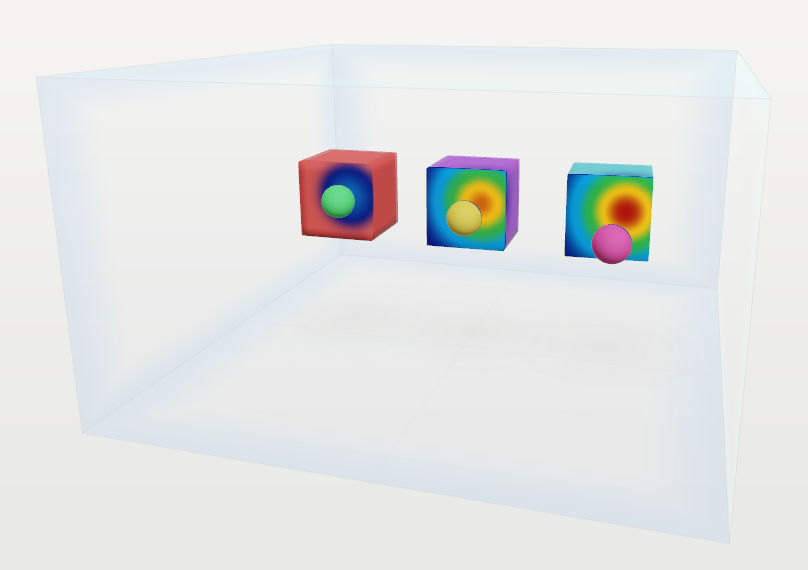
\includegraphics[width=.88\linewidth,height=78mm,keepaspectratio]{media/cuda-impact.png}
\caption{Urme de impact pe cele trei ținte. Albastrul și verdele
corespund intensităților mai mici, iar galbenul și roșul celor mai mari.}
\label{fig:impact}
\imagecredit{\path{media/cuda-impact.png}.}
\end{figure}
\begin{codefragment}{Calculează energia normală din viteza de apropiere și masa efectivă inversă.}{src/shared/sim/impacts.h}{60--64}
\begin{lstlisting}[numbers=left,firstnumber=60]
Real speed = maximum(0,  -dot(contactVelocity(s, ct.b_i, ct.point_m) - contactVelocity(s, ct.a_i, ct.point_m), ct.normal));

// Calculate the inverse of the effective mass along the normal.
Real inverse = effectiveMassInverse(s, ct, ct.normal);
return {speed, /* E = 0.5 * v^2 / m_inv */ inverse > settings::Collisions::Geometry::EPSILON ? HALF * speed * speed / inverse : 0};
\end{lstlisting}
\end{codefragment}

După rezolvare sunt păstrate evenimentele cu
\(v_c\geq0{,}5\,\mathrm{m/s}\), \(E_n\geq0{,}005\,\mathrm J\)
și impuls normal acumulat peste \(10^{-4}\,\mathrm{N\,s}\).
Fiecare object păstrează până la patru evenimente pe pas,
cu prioritate pentru cele cu energie mare.

\subsection{Collision heatmap}

Viewer-ul păstrează până la opt \emph{impact patches} pe object
sau pe o față a incintei. Punctul și normala sunt stocate în axele
locale ale object-ului, astfel încât urma se rotește odată
cu acesta. Pereții folosesc puncte proiectate pe suprafață.
Pentru energia \(E\) exprimată numeric în jouli, pragul de
saturație \(E_{\mathrm{red}}\), vârsta \(t\) și durata \(T\),
intensitatea urmei este
\begin{equation}
 H(E,t)=
 \clip\!\left(\frac{\ln(1+E)}{\ln(1+E_{\mathrm{red}})},0,1\right)
 \max(0,1-t/T)^{0{,}6}.
\end{equation}
Cu pragul de 10 J, o urmă nouă de 1 J are
\(\ln 2/\ln 11\approx0{,}29\), iar una de 10 J pornește de
la \(1\). Logaritmul face vizibile și loviturile slabe.
Urmele mai intense primesc raze mai mari, în limitele
stabilite de dimensiunea object-ului. Datele sunt pregătite
de \code{ImpactHistory::strength} și \code{ImpactHistory::advance}
(\coderef{src/client/render_gl/impact_history.cpp}{80--93, 140--165})
și transferate într-un \emph{shader storage buffer object} (SSBO).

Pentru un eșantion de suprafață în punctul local \(\vect x\)
cu normala \(\vect n\), pata cu centrul \(\vect p\), raza \(r_p\)
și normala \(\vect n_p\), contribuția unui \emph{impact patch} este
\begin{equation}
 H(E,t)\exp\!\left(-k\,\frac{\|\vect x-\vect p\|^2}{r_p^2}\right)
 \operatorname{smoothstep}(a,b,\vect n\cdot\vect n_p).
\end{equation}
Termenul de \emph{distance falloff} reduce intensitatea odată cu distanța.
Termenul de \emph{normal facing} reduce culoarea pe fețele întoarse
în altă direcție. Funcția GLSL \code{smoothstep(a, b, u)} transformă
valoarea \(u\) într-o pondere între 0 și 1, cu pragurile \(a<b\).
Întoarce 0 până la \(a\) și 1 de la \(b\) în sus. Între praguri
folosește o interpolare cubică Hermite \cite{glsl}.
\begin{equation}
 z=\clip\!\left(\frac{u-a}{b-a},0,1\right),
 \qquad \operatorname{smoothstep}(a,b,u)=3z^2-2z^3 .
\end{equation}
Panta în raport cu \(z\) este \(6z(1-z)\), deci trecerea începe
și se termină cu pantă zero. De exemplu, la un sfert din interval
ponderea este \(0{,}15625\), iar la trei sferturi este \(0{,}84375\).
În calculul \emph{normal facing}, \(u=\vect n\cdot\vect n_p\)
măsoară alinierea normalelor. Ponderea crește gradual când
suprafața se aliniază cu urma, astfel încât culoarea se estompează
la margine în loc să se schimbe brusc.
Fragment shader-ul păstrează intensitatea maximă dintre urmele suprapuse.
\begin{codefragment}{Combină distance falloff cu orientarea suprafeței pentru a calcula intensitatea urmei.}{src/client/render_gl/shaders/common/impact.glsl}{66--70}
\begin{lstlisting}[language=ReportGLSL,numbers=left,firstnumber=66]
vec3 delta = (local - pointRadius.xyz) / pointRadius.w;

float facing = smoothstep(WORLD.IMPACTS.IMPACT_FACING_LO, WORLD.IMPACTS.IMPACT_FACING_HI, dot(n, normalStrength.xyz));

return normalStrength.w * exp(-WORLD.IMPACTS.IMPACT_FALLOFF * dot(delta, delta)) * facing;
\end{lstlisting}
\end{codefragment}

Paleta împarte intervalul \([0,1]\) în patru segmente între
albastru, cyan, verde, galben și roșu. În fiecare segment,
\code{smoothstep(0.0, 1.0, u)} remapează poziția locală \(u\),
iar \code{mix} folosește ponderea rezultată pentru a combina
cele două culori de la capetele segmentului. Centrul unei urme
proaspete și saturate poate fi roșu, în timp ce marginile
aceleiași urme trec prin celelalte culori. Shaderul
amestecă paleta cu culoarea iluminată a object-ului.
\emph{Heatmap}-ul reprezintă severitatea impactului și estomparea
urmei pe suprafață.
\begin{codefragment}{Interpolează între culorile vecine ale paletei.}{src/client/render_gl/shaders/common/impact.glsl}{41--45}
\begin{lstlisting}[language=ReportGLSL,numbers=left,firstnumber=41]
vec3 impactPalette(float heat) {
    float ramp = clamp(heat, 0.0, 1.0) * 4.0;
    int i = min(int(ramp), 3);
    return mix(impactStop(i), impactStop(i + 1), smoothstep(0.0, 1.0, ramp - float(i)));
}
\end{lstlisting}
\end{codefragment}
\begin{codefragment}{Suprapune culoarea de impact peste culoarea iluminată.}{src/client/render_gl/shaders/body.frag}{141--145}
\begin{lstlisting}[language=ReportGLSL,numbers=left,firstnumber=141]
float heat = impactHeatAll(impactIndex, impactLocalPoint_m, impactLocalNormal, uImpactEnabled);
float key = max(dot(N, L_key), 0.0);

// Apply ACES tonemapping -> sRGB encoding -> impact heat -> final output.
fragmentColor = vec4(applyImpact(srgb(aces(result)), heat, key), 1.0);
\end{lstlisting}
\end{codefragment}

\section{Interfața viewer-ului}
\label{sec:viewer}

\begin{figure}[!htbp]
\centering
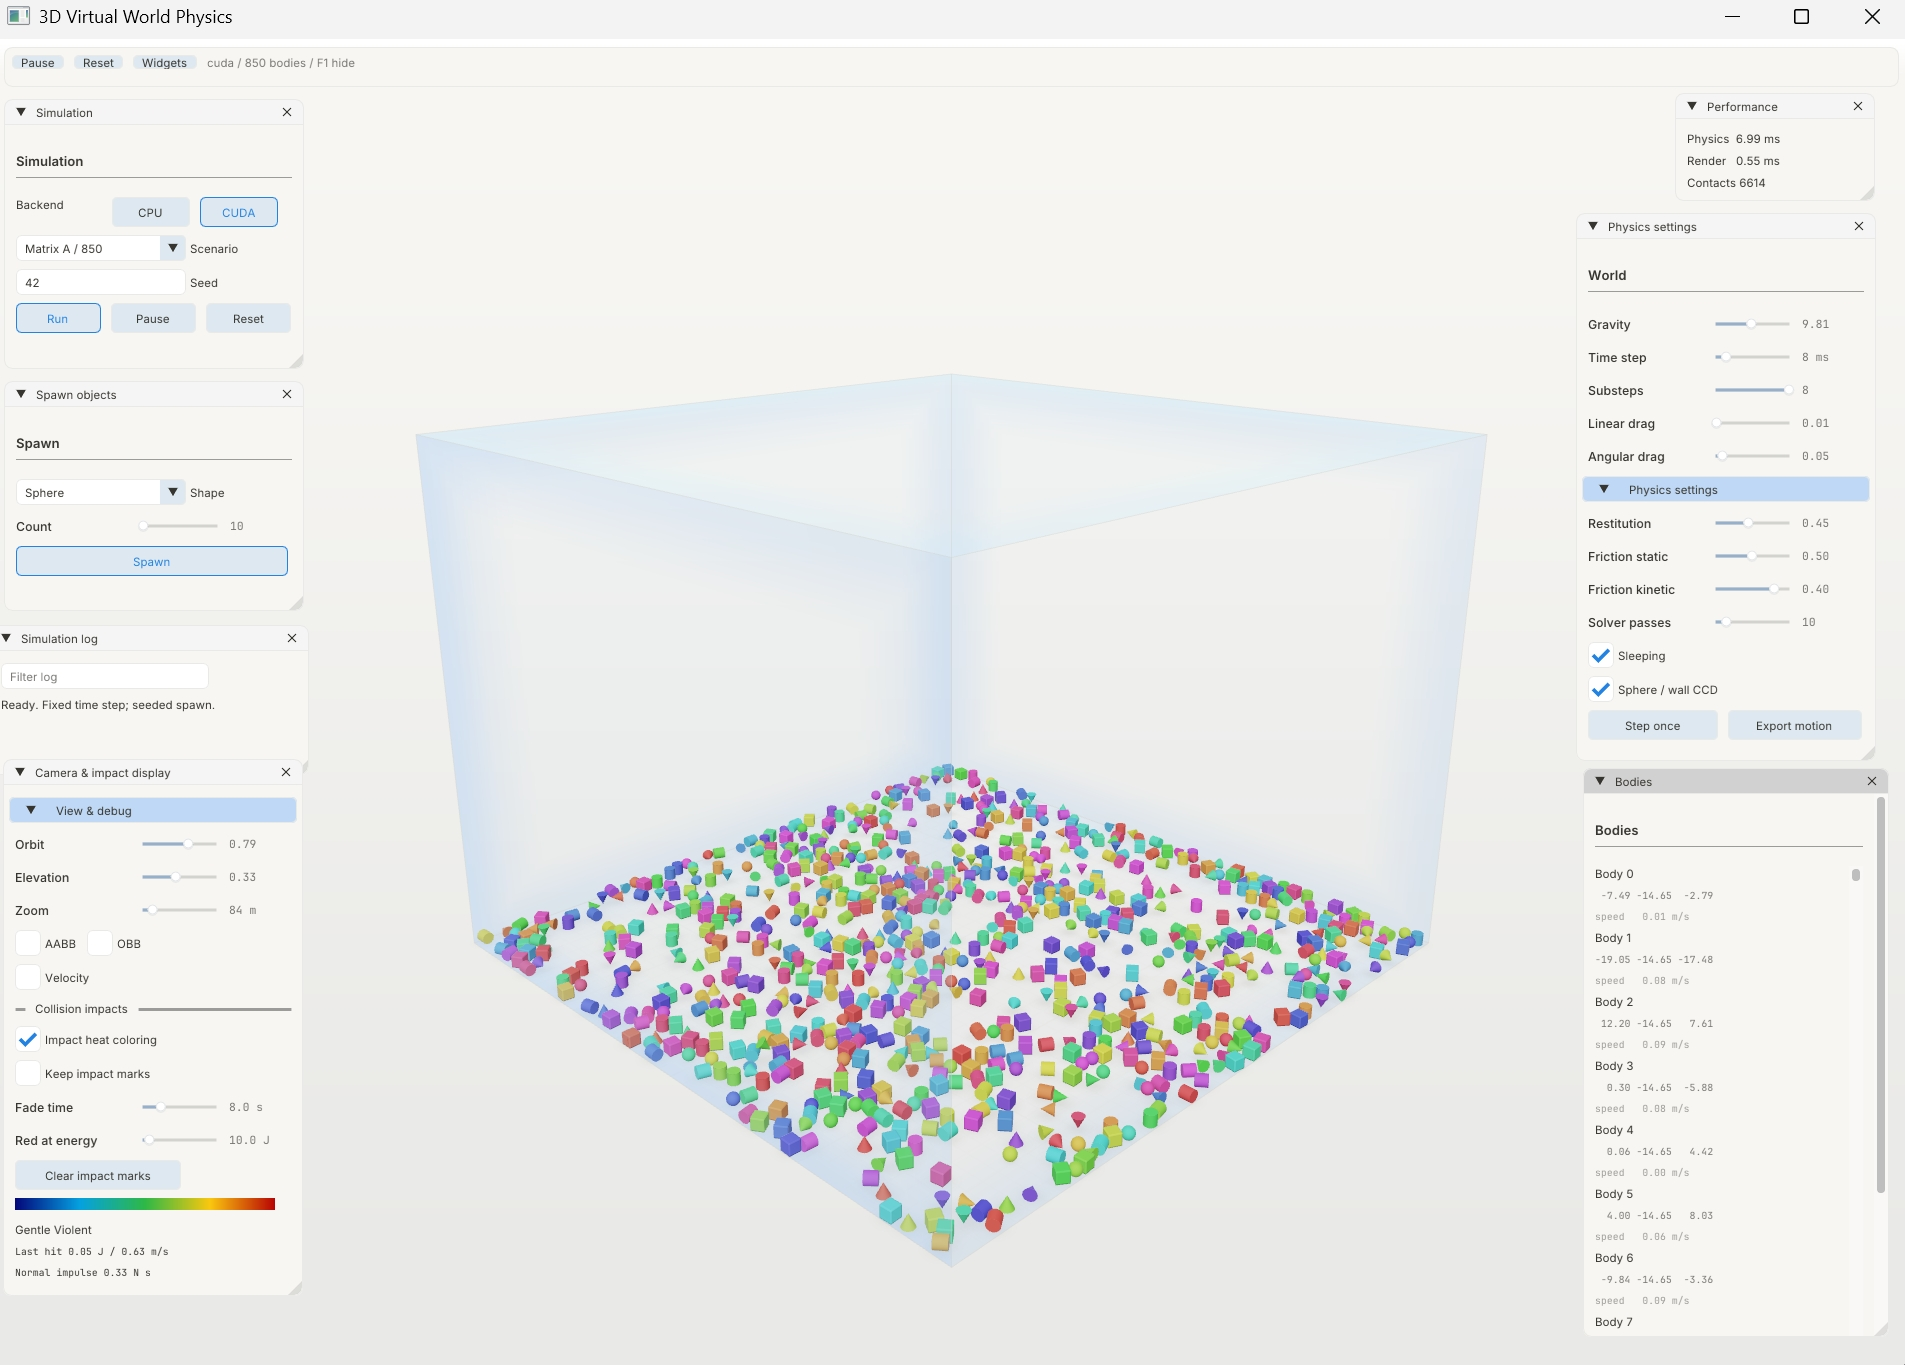
\includegraphics[width=\linewidth,height=113mm,keepaspectratio]{docs/figures/app_running.jpg}
\caption{Viewer-ul cu scena în centru, comenzile în stânga
și panourile de performanță și inspecție în dreapta.}
\label{fig:viewer}
\imagecredit{\path{docs/figures/app_running.jpg}.}
\end{figure}

Viewer-ul folosește Dear ImGui pentru \emph{widgets} și afișează
scena în același frame cu panourile din figura~\ref{fig:viewer}.
Butonul \emph{Widgets} comută vizibilitatea panourilor și oferă
control pentru dimensiunea textului. Tasta \code{F1} ascunde
sau afișează interfața.

\begin{description}
\item[Simulation.] \emph{Scenario} încarcă una dintre scene, iar
\emph{Seed} stabilește \emph{random seed}-ul folosit la inițializare.
\emph{Run} și \emph{Pause} controlează avansarea simulării,
iar \emph{Reset} recreează scena. Schimbarea din \emph{Backend}
copiază state-ul curent în noul backend, astfel încât poți continua
aceeași simulare pe CPU sau CUDA.
\item[Spawn objects.] Alegi \emph{Shape} și \emph{Count}, apoi
\emph{Spawn} adaugă objects în scena curentă. Dacă engine-ul
ajunge la limita de capacitate sau nu găsește o poziție validă
pentru următorul object, se oprește și scrie numărul adăugat în log.
\item[Physics settings.] \emph{Gravity}, \emph{Linear drag},
\emph{Angular drag}, \emph{Restitution}, \emph{Friction static}
și \emph{Friction kinetic} controlează dinamica.
\emph{Time step} este durata unui pas de simulare.
\emph{Substeps} limitează câți pași se pot executa într-un frame,
iar \emph{Solver passes} stabilește câte iterații de contact
se execută în fiecare pas. \emph{Sleeping} și \emph{Sphere / wall CCD}
activează comportamentele descrise în secțiunile de fizică.
\emph{Step once} execută un singur pas. \emph{Export motion} scrie
state-ul curent în \path{generated/reports/viewer/motion.csv}.
\item[Camera \& impact display.] \emph{Orbit}, \emph{Elevation}
și \emph{Zoom} mută camera. \emph{AABB}, \emph{OBB} și
\emph{Velocity} afișează debug overlays pentru limitele geometrice
și vectorii de viteză. \emph{Impact heat coloring} activează heatmap-ul.
\emph{Keep impact marks} oprește îmbătrânirea urmelor, \emph{Fade time}
stabilește durata lor, \emph{Red at energy} controlează pragul
de roșu, iar \emph{Clear impact marks} șterge urmele existente.
Legenda arată energia, viteza de apropiere și impulsul normal
pentru ultimul impact înregistrat.
\item[Performance, Bodies și Session log.] \emph{Performance} arată
timpul ultimului pas de simulare, timpul de render și numărul de
contacte. \emph{Bodies} este numele panoului în UI. Poți selecta
un object după ID și citi poziția și modulul vitezei.
\emph{Session log} afișează evenimente precum schimbarea backend-ului,
spawn și export, cu un câmp de filtrare.
\end{description}
Controalele și datele afișate sunt definite în
\coderef{src/client/physics_app/settings/parameter_windows.cpp}{87--130, 154--241, 278--405, 417--507}
și \coderef{src/client/physics_app/settings/diagnostic_windows.cpp}{34--52, 65--112}.
\begin{codefragment}{Comută vizibilitatea panourilor din meniul Widgets.}{src/client/physics_app/settings/parameter_windows.cpp}{395--399}
\begin{lstlisting}[numbers=left,firstnumber=395]
ImGui::MenuItem("Simulation", nullptr, &view.simulationWidget);
ImGui::MenuItem("Spawn objects", nullptr, &view.spawnWidget);
ImGui::MenuItem("Physics settings", nullptr, &view.physicsWidget);
ImGui::MenuItem("Camera & impact display", nullptr, &view.cameraWidget);
ImGui::MenuItem("Performance", nullptr, &view.performanceWidget);
\end{lstlisting}
\end{codefragment}

Pentru a urmări o singură coliziune, alegi scenariul de impact,
pui scena pe pauză și activezi săgețile de viteză și urmele.
\emph{Step once} avansează un pas. Săgețile arată schimbarea
mișcării, iar urmele arată locul impulsului confirmat.
\begin{codefragment}{Avansează simularea, descarcă starea și actualizează urmele.}{src/client/physics_app/run_session.cpp}{117--123}
\begin{lstlisting}[numbers=left,firstnumber=117]
void stepSimulation(Session& session) {
    session.backend->setImpactTracking(session.impacts().enabled);
    session.simulation.result = session.backend->step(session.simulation.state, session.scene.world);

    session.backend->download(session.simulation.state);
    session.impacts().advance(session.simulation.state, session.backend->impacts(), session.scene.world.dt_s);
}
\end{lstlisting}
\end{codefragment}

\section{Build și rulare}
\label{sec:build}

Proiectul folosește CMake 3.27 sau mai nou, Ninja, Git și un
compiler cu suport C++20. Pe Windows, scriptul de build detectează
MSVC și Windows SDK. Pentru CUDA sunt necesare un GPU NVIDIA,
driverul corespunzător și CUDA Toolkit 12.4 sau mai nou, cu un
host compiler acceptat de \code{nvcc}. Viewer-ul rulează cu OpenGL
4.6. Build-ul viewer-ului folosește Python 3 pentru generarea
loader-ului GLAD. CMake descarcă
dependințele prin \emph{FetchContent}, inclusiv nlohmann/json
și, pentru viewer, GLFW, GLM, GLAD și Dear ImGui.

\subsection{Build pe Windows}

Din directorul principal al proiectului, rulează în PowerShell.
\begin{lstlisting}[language=ReportPowerShell,numbers=left,firstnumber=1]
.\scripts\deployment\build-windows.ps1 -Cuda -Viewer -Architecture 89
.\exports\builds\windows-x64\physics_viewer.exe --backend cuda --scenario A
\end{lstlisting}
Scriptul configurează un \emph{Release build} cu Ninja în
\path{tmp/build/windows}. \code{-Cuda} activează
\code{ENABLE\_CUDA}, iar \code{-Viewer} activează
\code{BUILD\_VIEWER}. \code{-Architecture 89} selectează SM~89,
folosit în benchmark. Pentru alt GPU, alege valoarea
\emph{compute capability} corespunzătoare acelui model.
După build, directorul \path{exports/builds/windows-x64} conține
\code{physics.exe}, \code{physics\_viewer.exe} și DLL-urile de runtime
copiate de script.

\subsection{Build pe Linux}

Din directorul principal al proiectului, rulează în Bash.
\begin{lstlisting}[language=bash,numbers=left,firstnumber=1]
bash ./scripts/deployment/build-linux.sh --cuda --viewer --arch 89
./exports/builds/linux-$(uname -m)/physics_viewer --backend cuda --scenario A
\end{lstlisting}
Scriptul folosește \path{tmp/build/linux} ca \emph{build directory}
implicit și pune build outputs în \path{exports/builds/linux-} urmat
de arhitectura returnată de \code{uname -m}. Pentru un build
CPU-only, omite \code{-Cuda} pe Windows sau \code{--cuda} pe Linux
și pornește viewer-ul cu \code{--backend cpu}. Target-ul
\code{physics} este CLI-ul pentru benchmark și replay.
Target-ul \code{physics\_viewer} apare când build-ul include
viewer-ul. Configurarea și target-urile sunt definite în
\coderef{scripts/deployment/build-windows.ps1}{274--319},
\coderef{scripts/deployment/build-linux.sh}{150--183}
și \coderef{infra/Executable.cmake}{1--4, 30--42}.

\section{Validare experimentală}
\label{sec:evaluation}

\subsection{Metodă}

Executabilul Windows x64 a fost rulat în configurația Release
la 9 noiembrie 2026 pe un Intel Core i9-14900HX și un NVIDIA
GeForce RTX 4070 Laptop GPU. Versiunile au fost MSVC 19.51,
CUDA 13.4 pentru SM~89 și driverul 617.42. Starea a fost
reprezentată în precizie \code{float32}, cu \emph{random seed} 42
și pasul fix \(1/120\,\mathrm s\). Scenariul demonstrativ
a rulat \(2\,400\) de pași, iar matricile A, B și C câte 720.
Fiecare implementare a rulat independent din aceleași stări
inițiale. Figura~\ref{fig:matrices} arată cele trei densități.

\begin{figure}[!htbp]
\centering
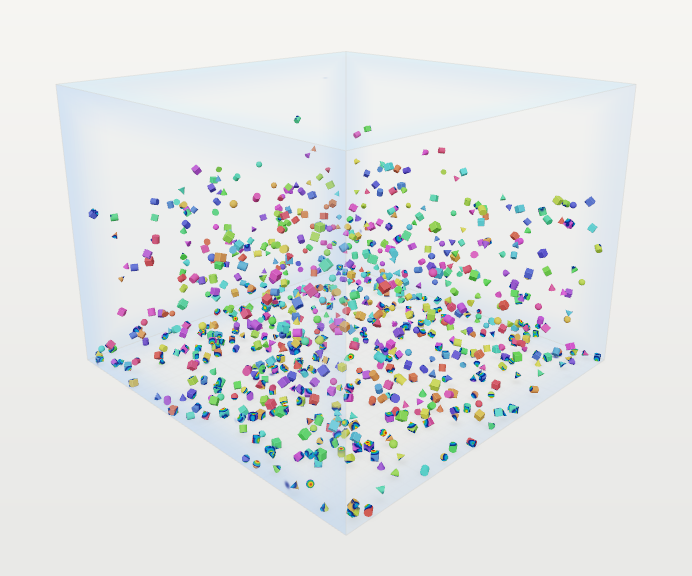
\includegraphics[width=\dimexpr\linewidth/3\relax]{media/matrices/cuda-A.png}%
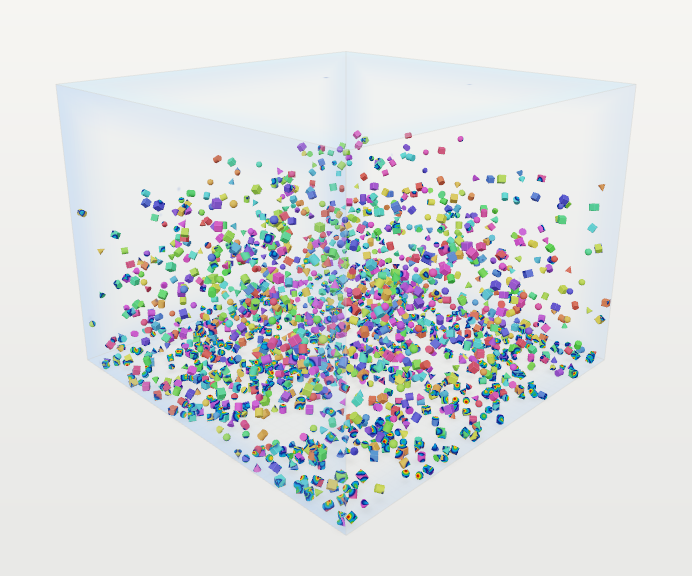
\includegraphics[width=\dimexpr\linewidth/3\relax]{media/matrices/cuda-B.png}%
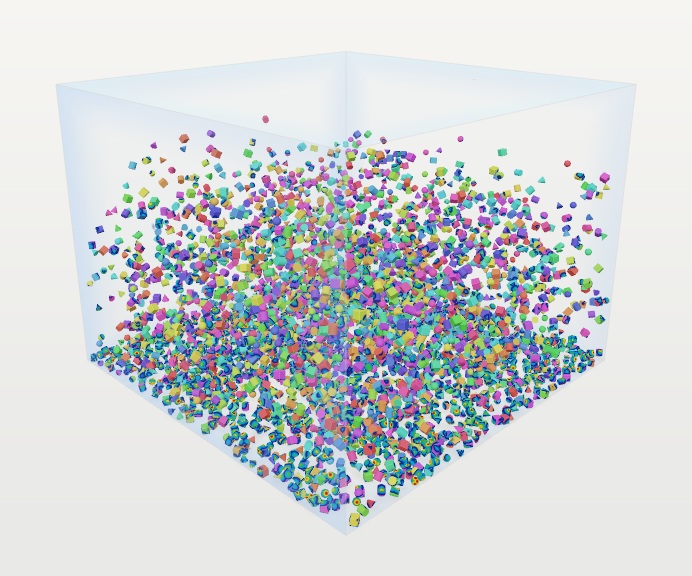
\includegraphics[width=\dimexpr\linewidth/3\relax]{media/matrices/cuda-C.png}
\caption{De la stânga la dreapta, matricile A, B și C, cu 850,
\(1\,750\) și \(4\,000\) de objects.}
\label{fig:matrices}
\imagecredit{\path{media/matrices/cuda-A.png}, \path{media/matrices/cuda-B.png}
și \path{media/matrices/cuda-C.png}.}
\end{figure}

Timpii provin din coloana \code{total\_wall\_ms} a fișierului
\path{frames.csv}. Măsurarea include primul pas și folosește
detectarea urmelor de impact dezactivată. Percentila 95 este
interpolată liniar între timpii ordonați. Timpii includ
sincronizarea diagnosticului CUDA. Descărcarea completă a
stării și randarea se măsoară separat de pasul fizic.

\subsection{Rezultate}

\begin{table}[!htbp]
\centering\small
\begin{tabular}{@{}lrrrl@{}}
\hline
\textbf{Scenariu} & \textbf{Objects} & \textbf{Pași identici}
  & \textbf{Contacte cumulate} & \textbf{Hash final} \\
\hline
Demo      & \(120\)     & \(2\,400/2\,400\) & \(1\,618\,414\)  & \code{15956118138859661966} \\
Matrice A & \(850\)     & \(720/720\)       & \(3\,153\,888\)  & \code{3330260331900169050} \\
Matrice B & \(1\,750\)  & \(720/720\)       & \(5\,966\,806\)  & \code{3349342891293941449} \\
Matrice C & \(4\,000\)  & \(720/720\)       & \(12\,165\,191\) & \code{11731164910491628103} \\
\hline
\end{tabular}
\caption{Comparație între CPU și CUDA. Contactele cumulate reprezintă
suma numărului de constrângeri pe toți pașii și coincid între implementări.}
\label{tab:parity}
\end{table}

Hash-urile coincid pentru toți cei \(4\,560\) de pași comparați.
La sfârșitul pașilor, ambele implementări au raportat zero ieșiri
din incintă. Diagnosticul nu a găsit poziții sau viteze nefinite.
Cea mai mare proiecție finală la un perete a fost de aproximativ
\(0{,}138\,\mathrm m\), în matricea B. Ea măsoară o corecție
geometrică din timpul pasului, iar ieșirile se verifică după corecție.

\begin{table}[!htbp]
\centering\small
\begin{tabular}{@{}lrrrrr@{}}
\hline
& \multicolumn{2}{c}{\textbf{CPU (ms/pas)}} &
  \multicolumn{2}{c}{\textbf{CUDA (ms/pas)}} & \\
\textbf{Scenariu} & Mediană & P95 & Mediană & P95 & \textbf{CPU/CUDA} \\
\hline
Demo      &  0,901 &  1,088 &  1,102 &  1,140 & \(0{,}82\) \\
Matrice A &  6,532 &  8,016 &  5,238 &  5,784 & \(1{,}25\) \\
Matrice B & 12,807 & 17,880 &  9,275 & 11,190 & \(1{,}38\) \\
Matrice C & 31,675 & 44,259 & 19,908 & 25,376 & \(1{,}59\) \\
\hline
\end{tabular}
\caption{Timpii pasului fizic. P95 este percentila 95, iar ultima coloană
este mediana CPU împărțită la mediana CUDA.}
\label{tab:timing}
\end{table}

În tabelul~\ref{tab:timing}, CUDA este mai rapid la toate cele
trei matrici. Scena cu 120 de objects favorizează CPU, deoarece
costul lansării și sincronizării CUDA cântărește mai mult când volumul
de calcul este mic. La matricea C, timpul pentru \emph{broad phase}
scade de la \(3{,}722\,\mathrm{ms}\) la \(0{,}616\,\mathrm{ms}\).
Rezolvarea contactelor rămâne etapa dominantă, cu mediane de
\(23{,}700\,\mathrm{ms}\) pe CPU și \(16{,}275\,\mathrm{ms}\) pe CUDA.
Diagnosticul serial CUDA are mediana \(2{,}781\,\mathrm{ms}\).
Medianele etapelor sunt calculate separat. Demo și matricea A
se încadrează la mediană în bugetul de \(8{,}33\,\mathrm{ms}\)
pe pas pe ambele implementări.

Testele unitare acoperă toate cele zece perechi de forme,
cei șase pereți, \emph{continuous collision detection} pentru sfere rapide,
repausul, reactivarea și reluarea deterministă. Comparația
CPU/CUDA cu cinci valori pentru \emph{random seed} a avut abatere finală nulă pentru
poziții și viteze. Testul CPU de un milion de pași pentru
o stivă a trecut, iar cutia de sus s-a stabilizat la
aproximativ \(3{,}1\,\mathrm{mm}\) sub poziția inițială.
Testele de impact au comparat și mișcarea cu și fără
înregistrarea urmelor.

\subsection{Reproducerea comparației}

După compilarea executabilului, rulează comenzile PowerShell
din directorul principal al proiectului. Înlocuiește
\code{A} cu \code{B} sau \code{C} pentru o scenă mai mare.
\begin{lstlisting}[language=ReportPowerShell,numbers=left,firstnumber=1]
$physics = '.\exports\builds\windows-x64\physics.exe'
$out = 'generated/reports/matrix-a-cpu'
$argsForRun = @('--backend','cpu','--scenario','A','--seed','42',
                '--ticks','720','--output',$out)
& $physics @argsForRun
& $physics --backend cuda --replay $out
\end{lstlisting}

Rularea scrie \path{config.json}, \path{initial.json},
\path{final.json}, \path{trace.csv}, \path{frames.csv},
\path{motion.csv} și \path{manifest.json}. Manifestul
include \emph{source fingerprint} în câmpul \code{sourceSha256}
și datele de execuție. La configurare, CMake calculează SHA-256
pentru fiecare fișier sursă și de configurare selectat, apoi
calculează SHA-256 din concatenarea acestor hash-uri
(\coderef{infra/SourceFingerprint.cmake}{5--13}).
O rulare separată cu \code{--backend cuda} și un director
propriu de ieșire produce timpii CUDA. \emph{Source fingerprint}
versiunii testate este
\begin{center}
  \small\code{257b984168a1014c5c034a6dcf075c1b3fd86f31a49f4038d688c9031ae7544e}
\end{center}

\section{Concluzii}

Rezolvarea contactelor în aceeași ordine permite folosirea
implementării CPU ca referință pentru CUDA. În scenele mai
mari, căutarea paralelă reduce timpul de detecție, iar
rezolvarea constrângerilor dintre objects rămâne costul
dominant. Viewer-ul leagă rezultatul fizic de imagine
prin orientarea object-urilor, umbrele de contact și urmele
de impact, fiecare calculată din datele pasului de simulare.

\section*{Sursele proiectului}
\addcontentsline{toc}{section}{Sursele proiectului}

Căile fragmentelor și ale imaginilor sunt relative la proiectul
\emph{Chasing the Moment of Impact} (\code{chasing-moment-of-impact}).
Fragmentele păstrează codul și numerotarea din sursă. Liniile
lungi sunt împărțite vizual pentru a încăpea în pagină.

\subsection*{Indexul surselor de cod}

Apasă pe un identificator din index pentru a reveni la fragmentul
sau la pasajul corespunzător. Identificatorul din text duce la
fișierul și intervalul de linii din index.

{\small
\begin{longtable}{@{}p{3em}
  >{\raggedright\arraybackslash}p{\dimexpr\linewidth-3em-9em-4\tabcolsep\relax}
  >{\raggedright\arraybackslash}p{9em}@{}}
\hline
\textbf{ID} & \textbf{Fișier sursă} & \textbf{Linii}\\
\hline
\endhead
\PrintCodeSources
\hline
\end{longtable}
}

% Bibliography
\bibliographystyle{plain}
\bibliography{references}

\end{document}